\documentclass[a4paper, 14pt]{extarticle}
\usepackage{graphicx}
\usepackage[T2A]{fontenc}
\usepackage[utf8]{inputenc}
\usepackage[russian]{babel}
\usepackage{setspace,amsmath}
\usepackage[left=20mm, top=15mm, right=15mm, bottom=15mm, nohead, footskip=10mm]{geometry} % Настройки полей документа

\graphicspath{ {./images/} }

\makeatletter
\def\@seccntformat#1{%
  \expandafter\ifx\csname c@#1\endcsname\c@section\else
  \csname the#1\endcsname\quad
  \fi}
\makeatother

\begin{document} % Начало документа

% Начало титульного листа
\begin{center}
    \normalsize{\textbf{МИНИСТЕРСТВО ОБРАЗОВАНИЯ РЕСПУБЛИКИ БЕЛАРУСЬ}}\\
    \hfill \break
    \normalsize{\textbf{БЕЛОРУССКИЙ ГОСУДАРСТВЕННЫЙ УНИВЕРСИТЕТ}}\\
    \hfill \break
    \small{\textbf{ФАКУЛЬТЕТ ПРИКЛАДНОЙ МАТЕМАТИКИ И ИНФОРМАТИКИ}}\\
    \hfill \break
    \large{Кафедра математического моделирования и анализа данных}\\
    \vspace{40mm}
    \normalsize{Курсовой проект}\\
    \hfill \break
    \normalsize{Криптография на основе функций хэширования:\\ подписи без состояния}\\
    \hfill \break
\end{center}

\begin{flushright}
    \vspace{20mm}
    Болтач Антон Юрьевич\\
    Студент 4 курса 9 группы\\
    Научный руководитель\\
    С. В. Агиевич\\
\end{flushright}

\vfill
\begin{center}
    Минск, 2019 г.
\end{center}
\thispagestyle{empty} % Выключаем отображение номера для этой страницы
    
% Конец титульного листа

\newpage

% Содержание
\tableofcontents
\newpage

% Введение
% Концепции Hash-based crypto
\section{Введение}
Цифровые подписи широко используются в Интернете, в частности, для аутентификации, проверки целостности и отказа от авторства. Алгоритмы цифровой подписи, наиболее часто используемые на практике - RSA, DSA и ECDSA, - основаны на допущениях твердости о задачах теории чисел, а именно факторизации составного целого числа и вычислении дискретных логарифмов. В 1994 году Питер Шор показал, что эти теоретические проблемы с числами могут стать решаемыми при наличии квантовых вычислений. Квантовые компьютеры могут решить их за полиномиальное время, ставя под угрозу безопасность схем цифровой подписи, используемых сегодня. Хотя квантовые компьютеры еще не доступны, их развитие происходит быстрыми темпами и поэтому представляет собой реальную угрозу в течение следующих десятилетий. К счастью, постквантовая криптография предоставляет множество квантовостойких альтернатив классическим схемам цифровой подписи. Подписи на основе хеша или подписи Меркле, как они также известны, являются одной из наиболее многообещающих из этих альтернатив.
\subsection{Почему Hash-Based Signatures?}
Есть много причин использовать схемы подписи на основе хеша и предпочитать их другим альтернативам. Хотя в самой ранней схеме подписи отсутствуют практические требования к производительности и пространству, современные схемы на основе хэшей, такие как XMSS, достаточно быстры, при небольшом размере. Также требования безопасности являются убедительными. Использование такой схемы подписи всегда требует хеш-функции. В то время как другие схемы подписи полагаются на дополнительные предположения о неразрешимости для генерации подписи, для решения на основе хеша требуется только безопасная хеш-функция. Некоторые схемы, основанные на хэше, даже уменьшают потребность в хэш-функции, устойчивой к столкновениям, до той, которая должна выдерживать атаки только на второе изображение. В качестве примера известны практические атаки средствами защиты от столкновений функции MD5, но мы до сих пор не знаем о виртуальных атаках на второе изображение.
\newpage

% Одноразовые подписи
\section{Одноразовые подписи(OTS)}
Одноразовые подписи (OTS) называются одноразовыми, поскольку сопутствующие сокращения безопасности гарантируют безопасность только при атаках с одним сообщением. Однако это не означает, что эффективные атаки возможны при атаках с двумя сообщениями. Особенно в контексте основанных на хэшировании OTS (которые являются основными строительными блоками последних предложений по стандартизации) это приводит к вопросу о том, приводит ли случайное повторное использование одноразовой пары ключей к немедленной потере безопасности. Проанализируем безопасность наиболее известных хэш-основанных OTS: WOTS, WOTS+ при различных видах атак с двумя сообщениями. Интересно, что оказывается, что схемы все еще безопасны при двух атаках сообщений, асимптотически.
\subsection{Одноразовая подпись Винтерница(WOTS)}
WOTS использует функцию сохранения длины (криптографический хэш) $F : \{0, 1\}^{n} \rightarrow \{0, 1\}^{n}$. Она параметризуется длиной сообщения $m$ и параметром $Winternitz$, $w \in N$, $w > 1$, который определяет компромисс между временем и памятью. Эти два параметра используются для вычисления
\[ l_{1} = \Bigg \lceil \frac{m}{log(w)} \Bigg \rceil, l_{2} = \Bigg \lfloor \frac{log(l_{1}(w - 1))}{log(w)} \Bigg \rfloor + 1, l = l_{1} + l_{2}. \]
Схема использует $w - 1$ итерации $F$ на случайном входе. Мы определяем их как
\[ F^{a}(x) = F(F^{a - 1}(x)) \]
и $F^{0}(x) = x$.

Теперь опишем три алгоритма схемы:

Алгоритм генерации ключей $(kg(1^{n}))$: На входе параметр безопасности $1^{n}$ алгоритм генерации ключей выбирает $l$ $n$-бит строки равномерно, случайным образом. Секретный ключ $sk = (sk_{1}, ..., sk_{l})$ состоит из этих $l$ случайных битовых строк. Открытый ключ проверки $pk$ вычисляется как
\[ pk = (pk_{1}, ..., pk_{l}) = (F^{w - 1}(sk_{1}), ..., F^{w - 1}(sk_{l})) \]

Алгоритм подписи$(sign(1^{n}, M^{*}, sk))$: На входе параметр безопасности $1^{n}$, сообщение $M^{*}$ длины $m$ и секретного ключа подписи $sk$, алгоритм подписи сначала вычисляет базовое $w$ представление $M^{*}: M^{*} = (M^{*}_{1}, ..., M^{*}_{l_{1}}), M^{*}_{i} \in \{0, ..., w - 1\}$. Далее он вычисляет контрольную сумму
\[ C = \sum^{l_{1}}_{i = 1}(w - 1 - M^{*}_{i}) \]

и вычисляет его базовое $w$ представление $C = (C_{1}, ..., C_{l_2})$. Длина базового $w$ представления $C$ не более $l_{2}$, так как $C \leq l_{1}(w - 1)$. Мы задаем $B = (B_{1}, ..., B_{l}) = M^{*} || C$. Подпись вычисляется как
\[ \sigma = (\sigma_{1}, ..., \sigma_{l}) = (F^{B_1}(sk_{1}), ..., F^{B_l}(sk_{l})) \].

Алгоритм проверки $(vf(1^{n}, M^{*}, \sigma, pk))$: На входе параметр безопасности $1^{n}$, сообщение $M^{*}$ длины $m$, подпись $\sigma$ и открытый ключ проверки $pk$, алгоритм проверки сначала вычисляет $B_{i}$, $ 1 \leq i \leq l$, как описано выше. Затем он выполняет следующее сравнение:
\[ pk = (pk_{1}, ..., pk_{l}) \stackrel{?}= (F^{w - 1 - B_{1}}(\sigma_{1}), ..., (F^{w - 1 - B_{l}}(\sigma_{l})) \]

Если сравнение выполняется, оно возвращает true и false в противном случае.
\subsection{Дополненная подпись Винтерница($WOTS^{+}$)}
Теперь опишем $WOTS^{+}$. Как и все варианты $W-OTS$, $W-OTS^{+}$ параметризуется параметром безопасности $n \in N$, длиной сообщения $m$ и параметром $w \in N$, $w > 1$, который определяет компромисс между временем и памятью. Последние два параметра используются для вычисления
\[ l_{1} = \Bigg \lceil \frac{m}{log(w)} \Bigg \rceil, l_{2} = \Bigg \lfloor \frac{log(l_{1}(w - 1))}{log(w)} \Bigg \rfloor + 1, l = l_{1} + l_{2}. \]

Кроме того, $W-OTS^{+}$ использует семейство функций $F_{n} : \{f_{k} : \{0, 1\}^{n} \rightarrow \{0, 1\}^{n}|k \in K_{n}\}$ с ключевым пространством $K_{n}$. Можно предположить как о криптографическом семействе хэш-функций, которое не сжимается. Используя $F_{n}$, мы определяем следующую цепную функцию.

$c^{i}_{k}(x, r):$ На входе значения $x \in \{0, 1\}^{n}$, счетчика итераций $i \in N$, ключа $k \in K$ и элементы рандомизации $r = (r_{1}, ..., r_{j}) \in \{0, 1\}^{nxj}$ при $j \geq i$, цепная функция работает следующим образом. В случае $i = 0$, $c$ возвращает $x(c^{0}_{k}(x, r) = x)$. Для $i > 0$ мы определяем $c$ рекурсивно как
\[ c^{i}_{k}(x, r) = f_{k}(c^{i - 1}_{k}(x, r) \oplus r_{i}) ,\]

То есть в каждом раунде функция сначала принимает побитовое $xor$ промежуточного значения и битовую маску $r$, затем оценивает $f_{k}$ на результат. Мы пишем $r_{a,b}$ для подмножества $r_{a}, ..., r_{b}$ как $r$. В случае $b < a$ мы определяем $r_{a,b}$ как пустую строку. Будем считать, что параметры $m$, $w$ и семейство функций $F_{n}$ общеизвестны. Теперь мы опишем три алгоритма $W-OTS^{+}$:

Алгоритм генерации ключа $(Kg(1^n))$: При вводе параметра безопасности $n$ в унарном, алгоритм генерации ключа выбирает $l + w - 1$ $n$-бит строки равномерно случайным образом. Секретный ключ $sk = (sk_{1}, ..., sk_{l})$ состоит из первых $l$ случайных битовых строк. Оставшиеся $w - 1$ бит строки используются в качестве элементов рандомизации $r = (r_{1}, ..., r_{w - 1})$ для $c$. Далее, $Kg$ выбирает функцию ключа $k \stackrel{\$}\leftarrow K$ равномерно случайным образом. Открытый ключ проверки $pk$ вычисляется как
\[ pk = (pk_{0}, pk_{1}, ..., pk_{l}) = ((r, k),c^{w - 1}_{k}(sk_{1},r), ..., c^{w - 1}_{k}(sk_{l}, r)). \]

Алгоритм подписи $(Sign(M, sk, r))$: На входе $m$ битного сообщения $M$, секретного ключа подписи $sk$ и элементов рандомизации $r$, алгоритм подписи сначала вычисляет базовое $w$ представление $M: M = (M_{1} . . . M_{l_{1}} )$, $M_{i} \in \{0, ..., w - 1\}$. Поэтому $M$ рассматривается как двоичное представление натурального числа $x$, а затем вычисляется $w$ бинарное представление $x$. Далее вычисляем контрольную сумму
\[ C = \sum^{l_{1}}_{i = 1}(w - 1 - M_{i}) \]

и его базовое $w$ представление $C = (C_{1}, ..., C_{l_{2}})$. Длина базового $w$ представления $C$ не более $l_{2}$, так как $C \leq l_{1}(w - 1)$. Мы задаем $B = (b_{1}, ..., b_{l}) = M || C$, конкатенация базовых $w$ представлений $M$ и $C$. Подпись вычисляется как
\[ \sigma = (\sigma_{1}, ..., \sigma_{l}) = (c^{b_{1}}_{k}(sk_{1},r), ..., c^{b_{l}}_{k}(sk_{l},r)). \]

Обратите внимание, что контрольная сумма гарантирует, что с учетом \newline
$b_{i}, 0 < i \leq l$, соответствующего одному сообщению, $b^{*}_{i}$ соответствующий любому другому сообщению включает по крайней мере один $b^{*}_{i} < b_{i}$.

Алгоритм проверки $(Vf(1^n, M, \sigma, pk))$: На входе сообщение $M$ двоичной длины $m$, подпись $\sigma$ и открытый ключ $pk$. Алгоритм проверки сначала вычисляет $b_{i}, 1 \leq i \leq l$, как описано выше. Затем он выполняет следующее сравнение:
\[ pk = (pk_{0}, pk_{1}, ..., pk_{l}) \stackrel{?}{=} ((r,k),c^{w - 1 - b_{1}}_{k}(\sigma_{1}, r_{b_{1} + 1, w - 1}, ..., c^{w - 1 - b_{l}}_{k}(\sigma_{l}, r_{b_{l} + 1, w - 1})) \]

Если сравнение выполняется, оно возвращает true и false в противном случае.

Время выполнения всех трех алгоритмов ограничено $lw$ оценками $f_{k}$. Размер подписи и секретного ключа составляет $|\sigma| = |sk| = ln$ бит. Размер открытого ключа равен $(l + w - 1)n + |k|$ бит, где $|k|$ обозначает количество бит, необходимых для представления любого элемента $K$.
\subsubsection{Обоснование стойкости($WOTS^{+}$)}
В этом разделе мы анализируем безопасность $WOTS^{+}$.

Определение($\epsilon$-доступность обнаружения подделки). $\epsilon$-доступность обнаружения подделки($\epsilon$-FDA) для одноразового $WOTS^{+}$ S определяется следующим экспериментом.
\newpage
Эксперимент $Exp^{F D A}_{S,n}(A)$

\hspace{10mm} $(sk, pk) \leftarrow S.Kg(1^n)$

\hspace{10mm} $(M^{*}, \sigma^{*}) \leftarrow A^{Sign(sk,\cdot)}$

Пусть $(M, \sigma)$ будьте парой запрос-ответ $Sign(sk,\cdot)$.

Вернём 1, если $S.Sign(sk, M^{*}) \rightarrow \sigma^{*}, S.Vf(pk, \sigma^{*}, M^{*}) \rightarrow 1, M^{*} \neq M$.

Тогда схема $WOTS^{*}$ $S$ имеет $\epsilon-FDA$, если нет противника $A$, который преуспевает с вероятностью $\geq \epsilon$.

Построим схему $(n, \delta, L, \nu)-W-OTS^{+}$ следующим образом.

Введем параметр $\nu \in \{1, 2, ...\}$ определение длины блоков, в которых сообщение разбивается во время алгоритма подписи, где мы предполагаем, что $L$ кратно $\nu$. Введем следующие вспомогательные значения:
\[w := 2^{\nu}, l_{1} := \lceil L/\nu \rceil, l_{2} := \lfloor log_{2}(l_{1}(w - 1))/\nu \rfloor + 1, l := l_{1} + l_{2}\].

Затем рассмотрим семейство односторонних функций:
\[ f^{(i)}_{r} : \{0,1\}^{n+\delta(w - i)} \rightarrow \{0,1\}^{n+\delta(w - i - 1)} \],

где $i \in {1, ..., w - 1}$ и параметр $r$ принадлежит некоторой области $D$. Мы предполагаем, что $f^{(i)}_{r}$ удовлетворяет случайному предположению оракула для равномерно случайно выбранного $r$ из $D$. Использование этого параметра может соответствовать $XOR$ некоторого семейства хэш-функций со случайной битовой маской.

Затем мы вводим цепную функцию $F^{(i)}_{r}$, которую мы определяем рекурсивно следующим образом:
\[F^{(0)}_{r}(x) = x, F^{(i)}_{r}(x) = f^{(i)}_{r}(F^{(i - 1)}_{r}(x)), i \in \{1, ..., w - 1\}.\]

Алгоритмы схемы $(n, \delta, L, \nu)-W-OTS^{+}$ следующие:

Алгоритм генерации пары ключей $((sk, pk) \leftarrow (n, \delta, L, \nu)-WOTS^{+}.Kg)$. Сначала алгоритм генерирует секретный ключ в следующем виде:
\[sk := (r, sk_{1}, sk_{2}, ..., sk_{l}), sk_{i} \stackrel{\$}{\leftarrow} \{0, 1\}^{n+\delta(w - 1)}, r \stackrel{\$}{\leftarrow} D\]
(Смотрите Рис. \ref{fig:wots1}). Затем открытый ключ, состоящий из рандомизирующего параметра $r$ и результаты цепной функции, используемой для $sk_{i}$ следующим образом:
\[ pk := (r, pk_{1}, pk_{2}, ..., pk_{l}), pk_{i} := F^{w - 1}_{r}(sk_{i})\]
Алгоритм подписи $(\sigma \leftarrow (n, \delta, L, \nu)-WOTS^{+}.Sign(sk, M))$. Сначала алгоритм вычисляет базовое $w$ представление $M$, разбивая его на $\nu$-битные блоки $(M = (m_{1}, ..., m_{l_{1}})$, где $m_{i} \in \{0, ..., w - 1\})$. Мы называем это частью сообщения. Затем алгоритм вычисляет контрольную сумму
\[ C := \sum^{l_{1}}_{i = 1}(w - 1 - m_{i}) \]
и его базовое $w$ представление $C = (c_{1}, ..., c_{l_{2}})$. Мы называем это контрольной суммой. Определим расширенную строку $B = (b_{1}, ..., b_{l}) := M||C$ как конкатенация частей сообщения и контрольной суммы. Наконец, подпись генерируется следующим образом:
\[ \sigma = (\sigma_{1}, ..., \sigma_{l}), \sigma_{i} := F^{(b_{i})}_{r}(sk_{i}). \]
Алгоритм проверки $(\nu \leftarrow (n, \delta, L, \nu)-WOTS^{+}.Vf(pk, \sigma, M))$. Идея алгоритма состоит в том, чтобы восстановить открытый ключ из заданной сигнатуры $\sigma$ и затем проверить, совпадает ли он с исходным открытым ключом $pk$. Во-первых, алгоритм вычисляет базовую $w$ строку $B = (B_{1}, ..., B_{l})$ таким же образом, как и в алгоритме подписи (см. выше). Затем для каждой части сигнатуры $\sigma_{i}$ алгоритм вычисляет оставшуюся часть цепочки следующим образом:
\[pk^{check}_{i} := f^{(w - 1)}_{r} \circ ... \circ f^{(b_{i}+1)}_{r}(\sigma_{i}),\]
где $\circ$ композиция функций. Если $pk^{check}_{i} = pk_{i}$ для всех $i \in \{1, ..., l\}$, затем алгоритм выводит $\nu := 1$, иначе $\nu := 0$.
\begin{figure}[h]
    \centering
    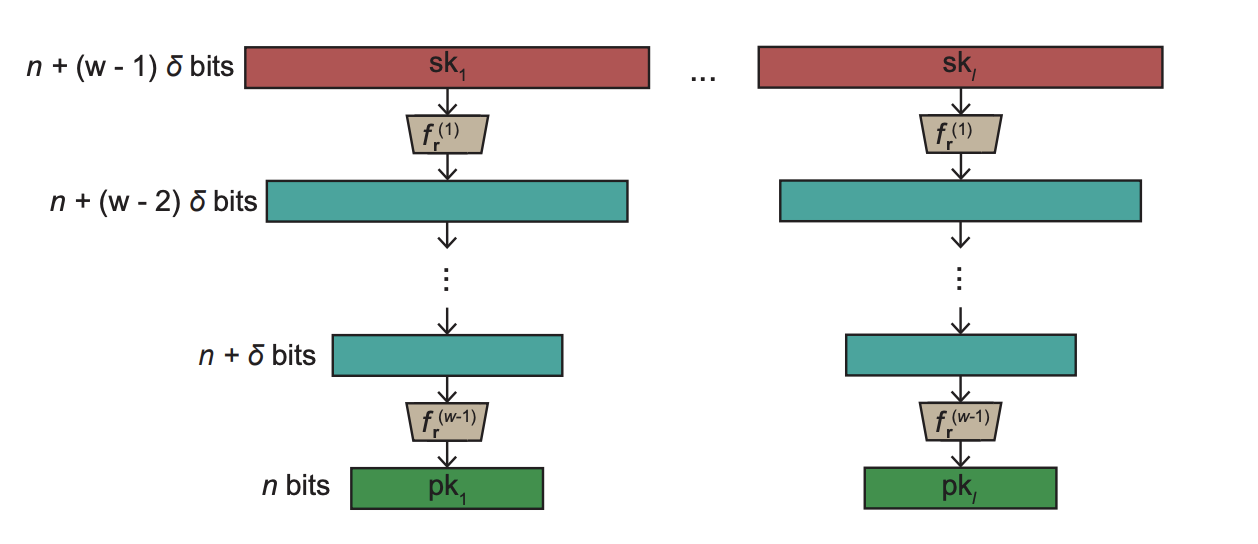
\includegraphics[scale=0.7]{WOTS+_1.png}
    \caption{Основной принцип построения открытого ключа в схеме $(n, \delta, L, \nu)-WOTS^{+}$ }
    \label{fig:wots1}
\end{figure}

Основной результат по свойству FDA схемы $(n, \delta, L, \nu)-W-OTS^{+}$ можно сформулировать следующим образом:
\newpage

% Деревья Меркля
\section{Деревья Меркля(MSS)}
Первый способ создать схему многократной подписи из схемы одноразовой подписи - использовать конструкцию, предложенную Мерклом в 1989 году. Учитывая целые числа $n$, $h$ и хэш-функцию $H$ : $\{0, 1\}^{2n} \rightarrow \{0, 1\}^{n}$, так называемое Дерево Меркля представляет собой двоичное дерево высоты $h$, узлы которого помечены значением $x \in \{0, 1\}^{n}$, таким образом, что значение каждого внутреннего узла вычисляется как $x = H(y||z)$, где $y$ и $z$ - значения левых и правых дочерних элементов.

Корневое значение $r$ может быть сначала отправлено для последующей аутентификации любого из $2^{h}$ листового значения $v_{1}, ..., v_{2^h}$. Действительно, чтобы проверить, что значение $v$ находится в листовом индексе $i$, нужно просто $v$, $i$ и путь аутентификации $i$. Этот путь аутентификации содержит братьев и сестер всех узлов на пути между листом $i$ и корнем (значения $h$). Это позволяет рекурсивно вычислять значения внутренних узлов вплоть до корня и сравнивать результат с $r$.

Эта конструкция позволяет превратить схему одноразовой подписи в схему многократной подписи следующим образом. Учитывая $2^h$ экземпляров OTS, подписывающий создает дерево Меркля, каждое листовое значение которого являются открытым ключом экземпляра OTS. Общий открытый ключ - это корневое значение. $i$-я подпись содержит подпись, сгенерированную $i$-м экземпляром OTS, а также путь аутентификации $i$.

Следовательно, открытый ключ содержит только $n$ битов, по сравнению с подходом $2^h$ OTS открытых ключей. Однако время генерации ключа экспоненциально в $h$, потому что на этом этапе необходимо вычислить полное дерево Меркля. Например, $h$ = 20 возможно, но может быть недостаточно для всех подписывающих. Кроме того, подписывающий должен отслеживать индексы $i$, которые уже были использованы, поэтому схема является $stateful$.
\newpage

% Многоразовые подписи
\section{Многоразовые подписи(MTS)}
В то время как одноразовые подписи обеспечивают удовлетворительную криптографическую безопасность для подписания и проверки транзакций, для них характерен существенный недостаток - их можно использовать безопасно только один раз. Поэтому существуют схемы подписи для включения более чем одной действительной одноразовой подписи, что позволяет сформировать предварительно столько подписей, сколько будет пар ключей одноразовых подписей. Логичным путем достижения этого является построение двоичного хеш-дерева, известного как дерево Меркля.
\subsection{HORS}
HORS - это простая схема подписи в несколько раз. Пусть $f$ - односторонняя функция, а $H$ - хэш-функция, которая выводит случайный размер подмножества $\{1,2,...,t\}$, где $k$ и $t$ - параметры, влияющие на безопасность с помощью $k < t$. Ключ подписи - это случайный кортеж $(s_1,...,s_t)$, а открытым ключом является $(f(s_{1}),..., f(s_{t}))$. 
Теперь, чтобы подписать $m$ сообщение, вычислить набор $S = H(m)$ и выходной $\{s_{i} : i \in S\}$. Чтобы проверить, примените $f$ к каждому элементу подписи и проверьте, соответствует ли он открытому ключу. Каждая подпись раскрывает $k$ элементы секретного ключа, поэтому в зависимости от выбора $k$ и $t$ несколько сообщений могут быть подписаны до того, как безопасность будет нарушена. Это было использовано в качестве строительного блока в SPHINCS, который представляет собой схему подписи на основе хэша без состояния, которая позволяет подписывать неограниченные сообщения.

\begin{figure}[h]
    \centering
    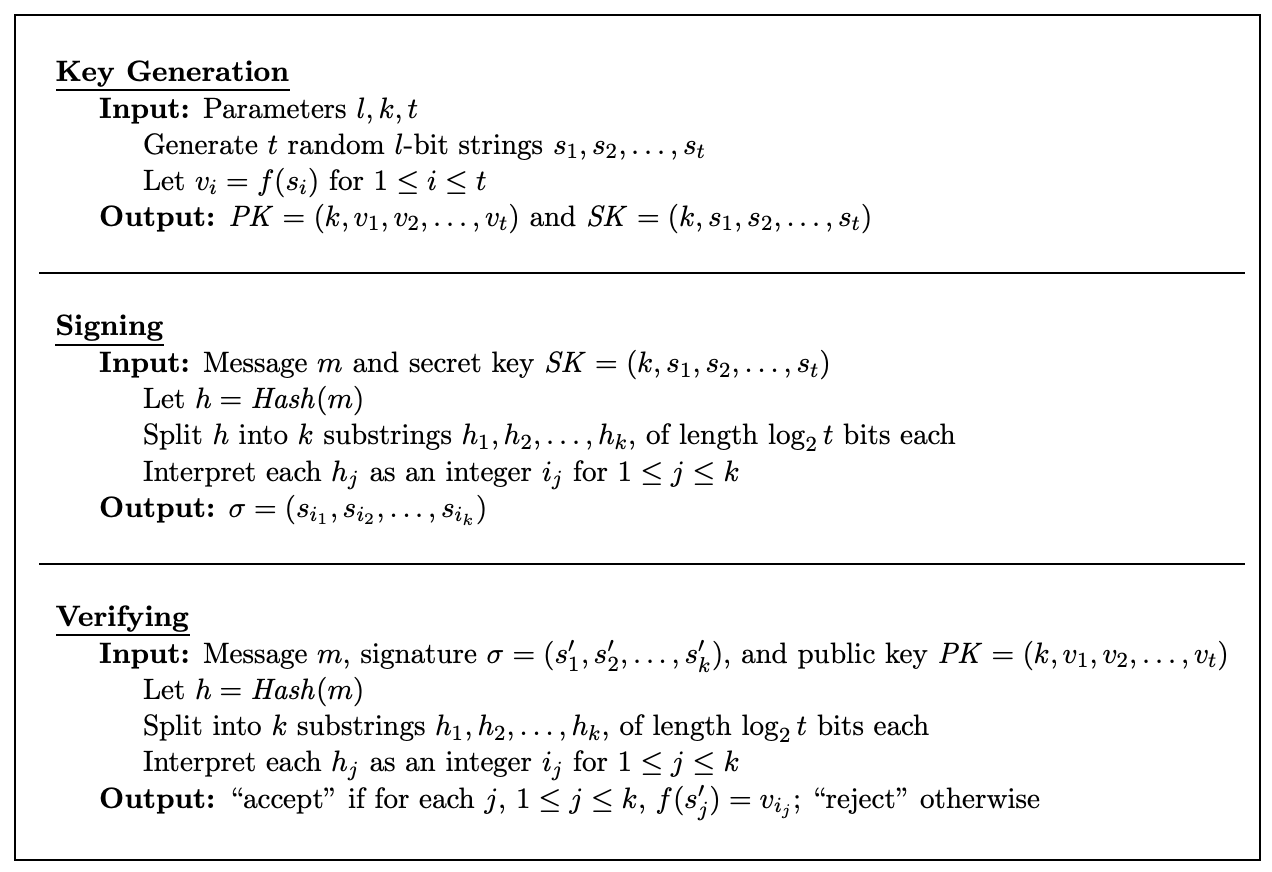
\includegraphics[scale=0.66]{HORS.png}
    \caption{Схема подписи HORS}
    \label{fig:hors}
\end{figure}
\subsection{PORS}
Начнём с того, что PORS, более безопасный вариант HORS. Как мы видели, современные схемы с несколькими временными подписями основаны на хэше для получения случайного подмножества (HORS). Тем не менее, HORS была изучена лишь частично, так как Рейзин и Рейзин(отец и сын) рассматривали только неадаптивные атаки. В частности, HORS подвержен адаптивным атакам, которые усугубляются простотой HORS: возьмите выход хэш-функции и разделите его на блоки, чтобы получить набор индексов. Действительно, ничто не мешает некоторым из этих индексов сталкиваться, уменьшая размер полученного подмножества и уменьшая безопасность. Несмотря на то, что HORS блестит своей простотой и скоростью по сравнению с более сложными методами получения случайных подмножеств гарантированного размера, его скорость не критична в сложных схемах, таких как SPHINCS, для которых голоса и деревья Меркля доминируют в вычислительных затратах. Поэтому рассмотрим новую конструкцию, использующую PRNG для получения случайного подмножества, которое мы называем PORS. Вместо того, чтобы использовать хэш-функцию, мы разделяем PRNG из сообщения и выполняем запрос к ней, пока мы не получим подмножество различных индексов к Рис. \ref{fig:pors}. Вычислительные издержки эквивалентны нескольким дополнительным вычислениям хэша для значительного повышения безопасности. В случае SPHINCS заметим, что противники имеют полный контроль над выбранным листом в гипердереве. Вместо этого мы предлагаем создать этот листовой индекс с помощью PRNG, что ещё больше повысит уровень безопасности. Этот увеличенный запас прочности позволяет уменьшить высоту гипердерева на 2 слоя, экономя 4616 байт.

\begin{figure}[h]
    \centering
    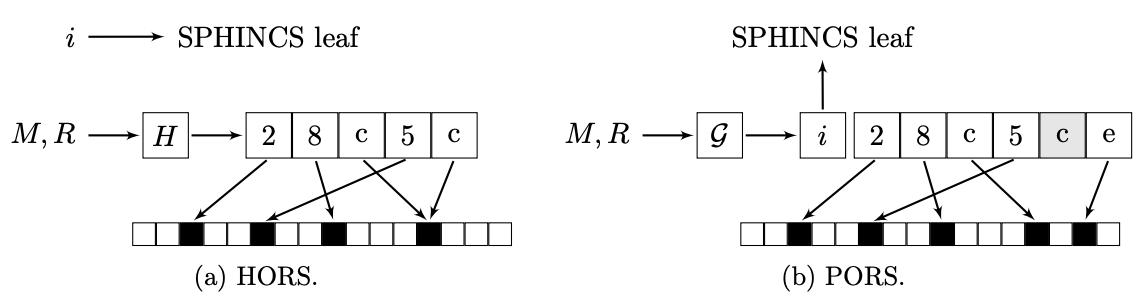
\includegraphics[scale=0.85]{PORS.png}
    \caption{Сравнение HORS и PORS}
    \label{fig:pors}
\end{figure}
\newpage

% Подписи без состояния
\section{Подписи без состояния}
\subsection{SPHINCS}
\subsection{Gravity-SPHINCS}
\subsection{SPHINCS+}

% Сравнение Stateful && Stateless
\section{Stateful vs Stateless}
Схемы с сохранением состояния имеют дерево Меркля с количеством одноразовых подписей внизу. Каждая разовая подпись может быть использована один раз, следовательно, подписывающий должен отслеживать, какие из них он использовал. То есть, когда он использует одноразовую подпись для подписи сообщения, он должен обновить свое состояние.

Схемы без состояния имеют большое дерево, но внизу у них есть несколько подписей времени. Каждая такая небольшая временная подпись может подписать несколько сообщений. Таким образом, когда подписывается сообщение, подписывающий выбирает случайную подпись с небольшим количеством времени, использует ее для подписи сообщения, а затем подтверждает ее подлинность через деревья Меркля вплоть до корня, который является открытым ключом. Поскольку мы используем несколько раз подпись, мы не против, если мы иногда выбираем одну и ту же подпись несколько раз. Схема подписи нескольких раз может справиться с этим. И, поскольку нам не нужно обновлять какое-либо состояние при генерации подписи, это считается «без сохранения состояния».
\newpage

% Заключение
\section{Заключение}
\newpage

% Литература
\section{Литература}
\newpage


\end{document}
% Конец документа